% Die Beamer-Klasse unterstützt folgende Optionen, die von
% besonderem Interesse sind (alle Standardoptionen werden
% ebenfalls unterstützt; siehe beamer-Basisdokumentation):
% 
%%%%%%%%%%%%%%%%%%%%%%%%%%%%%%%%%%%%%%%%%%%%%%%%%%%%%%%%%%%%%%%
% aspectratio: Seitenverhältnis des resultierenden Dokuments
% (Achtung: Aufgrund der Designvorgaben ergeben sich unterschiedliche
% Größen der effektiv nutzbaren Textblöcke)
%
% Standardeinstellung: 'aspectratio=43'
%
% Mögliche Einstellungen:
% 'aspectratio=43'   (4:3)
% 'aspectratio=169'  (16:9)
% 'aspectratio=1610' (16:10)
% 
%%%%%%%%%%%%%%%%%%%%%%%%%%%%%%%%%%%%%%%%%%%%%%%%%%%%%%%%%%%%%%%
% fontsize: Basisschriftgröße (Größen für Überschriften etc. werden
% aus dieser Basis automatisch abgeleitet)
%
% Standardeinstellung: '22pt' (entspricht den Design-Vorgaben; sehr groß!)
%
% Mögliche Einstellungen:
% '8pt', '9pt', '10pt', '11pt', '12pt', '14pt', '16pt',
% '17pt','20pt','22pt', '24pt', '26pt', '28pt'

\documentclass[aspectratio=169,16pt,xcolor=table]{beamer}

% Der OTHR-Theme unterstützt folgende Optionen:
% 
%%%%%%%%%%%%%%%%%%%%%%%%%%%%%%%%%%%%%%%%%%%%%%%%%%%%%%%%%%%%%%%
% department: (Wahl der Abteilung/Fakultät)
%
% default: 'OTHR'
%
% Mögliche Einstellungen:
% 'FakA', 'FakAM', 'FakB', 'FakBW', 'FakEI', 
% 'FakIM', 'FakM', 'FakS', 'ZWW', 'IPF',
% 'SappZ', 'KNB', 'ReMIC', 'LFD', 'LAS3',
% 'DK0PT', 'LBM', 'LeanLab', 'LFT', 'LFW',
% 'LMP', 'LMS', 'LRT', 'LWS', 'RRRU',
% 'RST', 'CEEC', 'FEM', 'IST'
%%%%%%%%%%%%%%%%%%%%%%%%%%%%%%%%%%%%%%%%%%%%%%%%%%%%%%%%%%%%%%%%%
% headerMode: Aussehen und Inhalt der Kopfleiste
%
% Standardeinstellung: 'full'
%
% Mögliche Einstellungen:
% 'full', 'frametitle', 'frametitleSection'
% 

%%%%%%%%%%%%%%%%%%%%%%%%%%%%%%%%%%%%%%%%%%%%%%%%%%%%%%%%%%%%%%%%%
% Binäre Schalter (können angegeben oder nicht angegeben werden;
% Standardeinstellung: Nicht angegeben)
%
%%%%%%%%%%%%%%%
% navbar: Navigationssymbole anzeigen (Seite vor/zurück, Kapitel vor/zurück etc.)

% pageNumbers: Seitennummerierung

% blackFont: Nur schwarze Schriftfarbe verwenden (ansonsten: Fakultätsfarben)

% frametitleCenter: Titel in der Kopfzeile zentrieren (ansonsten: rechtsbündig)

\usetheme[department=FakIM,pageNumbers]{OTHR}

% Inhaltsspezifische Zusatzpakete laden 
\usepackage[ngerman]{babel}
\usepackage[utf8]{luainputenc}
\usepackage{lipsum}
\usepackage{graphicx}
\graphicspath{ {./img/} }
\usepackage{amsmath}
\usepackage{adjustbox}
\usepackage{xcolor}
\usepackage{ulem}
\usepackage[usestackEOL]{stackengine}
\usepackage{hyperref}
\usepackage{biblatex}
\usepackage{breakcites}
\usepackage{etoolbox}

\renewcommand\bibfont{\tiny}
\addbibresource{ref.bib}

\patchcmd{\thebibliography}{\footnotesize}{\tiny}{}{}

% this adds the content table for each section
\AtBeginSection[]
{
  \begin{frame}
    \frametitle{Inhalt}
    \tableofcontents[currentsection]
  \end{frame}
}

\date{15. Januar 2024}

\begin{document}

\begin{frame}{YouTube Video Vorschau}
    \centering
    \href{https://www.youtube.com/watch?v=PLk8Pm_XBJE&t=612s}{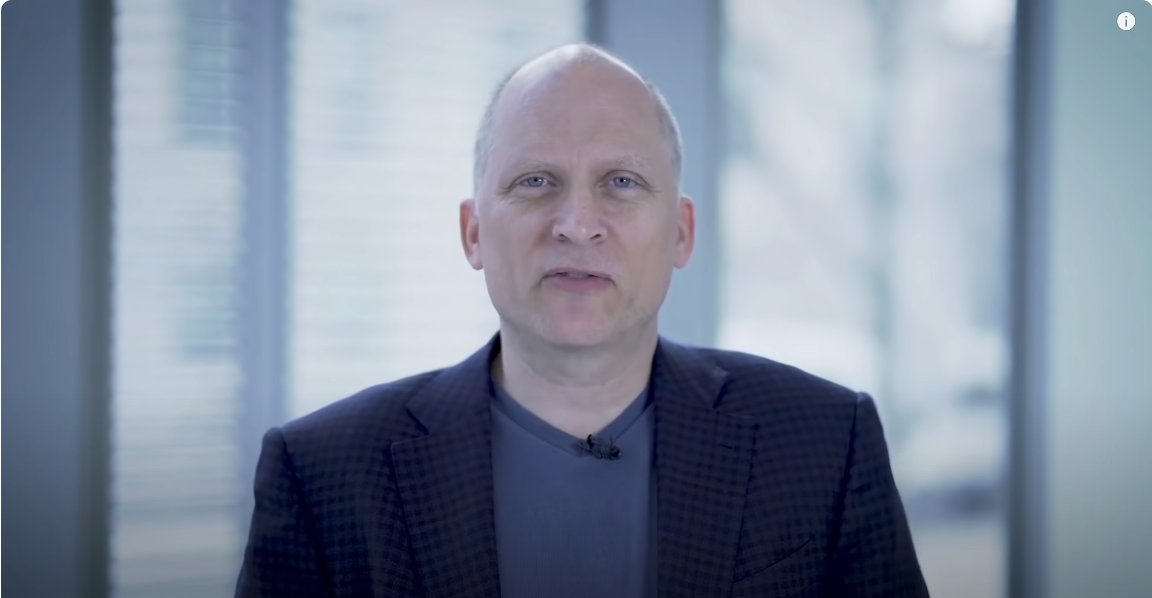
\includegraphics[width=0.8\linewidth]{pictures/Video_Vorschau.png}}
    \vspace{-0.2cm}
    \begin{flushleft}
        \tiny Quelle: \url{https://www.youtube.com/watch?v=PLk8Pm_XBJE}, zuletzt besucht am 12.12.2023
    \end{flushleft}
\end{frame}

\title{Transhumanismus}
\subtitle{Fortschritt oder Dystopie?}
\author{Marcel Ott, Nicolas Zander, Lorenz Branner, Severin Bittl, Thomas Gailinger}
\institute{Ethik in der Informatik}

\maketitle

%\begin{frame}
%	\frametitle{Inhaltsverzeichnis}
%	\tableofcontents
%\end{frame}

\section{Einleitung}
\subsection{Begriffserleuterungen}
\begin{frame}
	\frametitle{Begriffserleuterungen}
	\begin{itemize}
	  \item Transhumanismus
    \begin{itemize}
      \item Ausschöpfung der natürlichen menschlichen Grenzen mit Wissenschaft~\cite{Merzlyakov2022}\\
      => Beibehaltung der Grundform des Menschen
    \end{itemize}
	\item Posthumanimus
    \begin{itemize}
      \item Überwindung der menschlichen Grenzen~\cite{Merzlyakov2022}\\
      \item Mensch ist eine Sackgasse und Cyborg wird als nächster Schritt der Evolution angesehen~\cite{Merzlyakov2022}\\
      => Grundform des Menschen wird abgeschafft
    \end{itemize}
	\item Cyborg
    \begin{itemize}
      \item Integriertes System aus menschlichen und maschinellen Teilen~\cite{warwick2000cyborg}
    \end{itemize}
	\end{itemize}
\end{frame}

\subsection{Was ist normal?}
\begin{frame}
  Breczko: Die Überwachung biotechnologischer Möglichkeiten erfordert zweifellos eine Unterschiedung zwischen „therapeutischen“ und „Verbesserungs“-Aktivitäten~\cite{breczko2021human}\\
  => Was ist normal?
\end{frame}

\begin{frame}
	\begin{itemize}
	  \item Statischer Durchschnitt oder 
    \begin{itemize}
      \item 
    \end{itemize}
  \end{itemize}
\end{frame}


\section{Ethische Fragestellungen des Transhumanismus}
\subsection{Selbstbestimmung des Individuums}
\begin{frame}
  \frametitle{Selbstbestimmung des Individuums}
  \begin{itemize}
    \item \textbf{Recht auf freie Entfaltung:} Jeder hat das Recht auf freie Entfaltung, solange die Rechte anderer oder bestehendes Recht nicht verletzt werden\cite{fur1996grundgesetz}.
    \begin{itemize}
      \item \textit{Individuelle Identität:} Menschen können ihre eigene Identität frei wählen.
      \item \textit{Natürlichkeit bewahren:} Der Wunsch, in seiner natürlichen Form zu bleiben, ist ein essentieller Aspekt.
    \end{itemize}
    \item \textbf{Freie Entscheidung in einer Welt der Verbesserung:} In einer Gesellschaft, in der die Mehrheit von Enhancements profitiert, könnten jene, die sich dagegen entscheiden, im Alltagsleben benachteiligt sein (z.B., Profi Bodybuilding und der Einsatz von Steroiden).
  \end{itemize}
\end{frame}


\subsection*{Entscheidungen Treffen für Andere}
\begin{frame}
  \frametitle{Entscheidungen Treffen für Andere}
  \begin{itemize}
    \item Schwierigkeit der Entscheidungsfindung für andere in Bezug auf Verbesserungen\cite{plavsienkova2021healthy}.
    \item Individuelle Abwägung von Nebenwirkungen: Jeder muss für sich selbst entscheiden, ob er die möglichen Nebenwirkungen in Kauf nehmen möchte.
    \item Gesellschaftliche Verantwortung: Die Gesellschaft könnte die Konsequenzen tragen, wenn Menschen sich gegen Verbesserungen entscheiden, z.B., höhere Gesundheitskosten und zusätzliche Kosten für die Integration ins tägliche Leben. Dies könnte zu einer Pflicht zur Verbesserung führen.
    \item Herausforderung bei nicht selbstbestimmter Entscheidung: Besonders kritisch wird es bei Menschen, die nicht selbstbestimmt entscheiden können. Beispiel: Locked-in-Syndrom, bei dem die Betroffenen denken und fühlen können, aber nicht sprechen oder sich bewegen können\cite{das2022locked}.
    \item Einschränkungen durch Entscheidungen für Andere: Entscheidungen gegen Verbesserungen könnten zu späteren Einschränkungen in der Teilhabe am Gemeinschaftsleben führen.
  \end{itemize}
\end{frame}

\subsection*{Fallbeispiel: Entscheidung für ein Kind}
\begin{frame}
  \frametitle{Fallbeispiel: Entscheidung für ein Kind}
  \begin{itemize}
    \item Gerichtsverhandlung wegen Entscheidung gegen ein Cochlea-Implantat bei gehörlosen Eltern\cite{brde}.
    \item Die Klinik sah die Ablehnung als Gefährdung des Kindeswohls und leitete ein Kinderschutzverfahren ein.
    \item Familiengerichtsentscheidung am 29. Januar 2019:
    \begin{itemize}
      \item Keine familienrechtlichen Maßnahmen aufgrund unzureichender Gründe.
      \item Eltern können den optimalen Therapieverlauf nach der Implantation nicht gewährleisten.
      \item Ohne Akzeptanz der Eltern ist es unmöglich, dass das Kind trotz Cochlea-Implantat die Hör- und Sprachfähigkeit erlangt.~\cite{brde}
    \end{itemize}
  \end{itemize}
\end{frame}


\subsection*{Autonomie einer Gruppe}
\begin{frame}
  \frametitle{Autonomie einer Gruppe}
  \begin{itemize}
    \item Möglichkeit zur ``Normalität'' für Minderheiten: Die Gefahr besteht, dass die Anliegen derjenigen, die sich gegen Normalisierung entscheiden, weniger Beachtung finden, da sie nicht mehr als Teil einer diskriminierten Gruppe betrachtet werden (Argument der leichteren Lösung).
    \item Erhaltung kultureller Dynamik: Minderheiten und Gruppen haben ihre eigene kulturelle Dynamik, die durch Normalisierung verloren gehen könnte. Beispiel: Gehörlosen-Community, die eine einzigartige Kommunikationsform pflegt und geschätzt werden sollte\cite{lee2016cochlear}.
    \item Gewinn an Autonomie für Betroffene Gruppen: Durch Technologie könnten betroffene Gruppen wieder selbstbestimmter leben\cite{das2022locked}.
  \end{itemize}
\end{frame}

\subsection*{Unabschätzbare Folgen}
\begin{frame}
  \frametitle{Unabschätzbare Folgen}
  \begin{itemize}
    \item \textbf{Beispiel aus der Vergangenheit:} FCKW als Kältemittel und Treibmittel in Spraydosen führten zur Entstehung des Ozonlochs\cite{rowland1996stratospheric}.
    \item \textbf{Transhumanismus und Posthumanismus:} Unvorhersehbare Folgen im eigenen Körper, insbesondere bei DNA-Veränderungen, könnten fatale und irreversible Auswirkungen haben. Obwohl die DNA-Forschung fortgeschritten ist, bleiben viele ungeklärte Fragen, was zu potenziell fatalen Fehlern führen könnte.
    \item \textbf{Beispiel: Deep Brain Stimulation (DBS):} Elektroden im Gehirn, die elektrische Impulse abgeben, können therapeutische Effekte haben. Komplexität des Gehirns führt zu unerwünschten Nebenwirkungen wie Depressionen oder Suizid bei Empfängern von DBS\cite{zarzycki2020stimulation}.
    \item \textbf{Herausforderungen bei DBS:} Elektroden stimulieren großflächig, was zu ungewollten Stimulationen benachbarter Gehirnareale führen kann. Kleine Änderungen in Intensität oder Zeitverzögerung können unvorhersehbare Auswirkungen haben\cite{al2021impact}. Tierversuche mit Affen zeigten, dass Änderungen in Frequenz und Platz der Stimulation zu gegenteiligen Effekten führen\cite{logothetis2010effects}.
  \end{itemize}
\end{frame}


\section{Risikoberwertung}
\subsection{Regulierungen}
\begin{frame}{Regulierungen}
Regulierungen
	\begin{itemize}
		\item{Regulierungen, rechtliche Rahmenbedingungen und Ethikcodizes nötig}
		\item{AI Act der EU 2021~\cite{ai_act_eu_2021} und Fortschritte damit~\cite{ai_act_deal_2023}}
		\item{Seit einigen Jahren im Diskurs anhand vergleichbarer Fälle~\cite{lee2016cochlear}}
	\end{itemize}
\end{frame}

\subsection{Risiken}
\begin{frame}{Risiken}
Risiken
	\begin{itemize}
		\item{Einteilung in Individuum, Organisationen und Gesellschaft}
	\end{itemize}
\end{frame}

\subsubsection{Individuum}
\begin{frame}{Risiken - Individuum}
Risiken - Individuum
	\begin{itemize}
		\item{Folgen von Hackerangriffen~\cite{khan_aziz_2019}}
		\item{Eigengefährdung von Nutzenden~\cite{khan_aziz_2019}}
		\item{Gefahren bei Operationen~\cite{Burwell:2017aa}}
		\item{Unbekannte Langezeitfolgen~\cite{Burwell:2017aa}}
	\end{itemize}
\end{frame}

\subsubsection{Organisationen}
\begin{frame}{Risiken - Organisationen}
Risiken - Organisationen
	\begin{itemize}
		\item{Kapitalgetriebene Entscheidungen~\cite{khan_aziz_2019}}
		\item{Neuro-Marketing~\cite{khan_aziz_2019}}
		\item{Monopolbildung~\cite{khan_aziz_2019}}
	\end{itemize}
\end{frame}

\subsubsection{Gesellschaft}
\begin{frame}{Risiken - Gesellschaft}
Risiken - Gesellschaft
	\begin{itemize}
		\item{Unfairen Vorteil verschaffen~\cite{khan_aziz_2019}}
		\item{Militante Interessen~\cite{khan_aziz_2019}}
		\item{Verlust Autonomie und Menschlichkeit~\cite{Burwell:2017aa}}
	\end{itemize}
\end{frame}

\subsection{Risikoeinordnung}


\newpage
\printbibliography % Druckt das Literaturverzeichnis in kleinerer Schriftgröße aus

%=======
\section{Lorenz}
\subsection{Gesundheit}
\begin{frame}
	\frametitle{Basics}
	\begin{itemize}
	\item Test
	\end{itemize}
\end{frame}
%>>>>>>> main
\end{document}
